\documentclass{standalone}
\usepackage{tikz}
\usetikzlibrary{angles,quotes}

\begin{document}

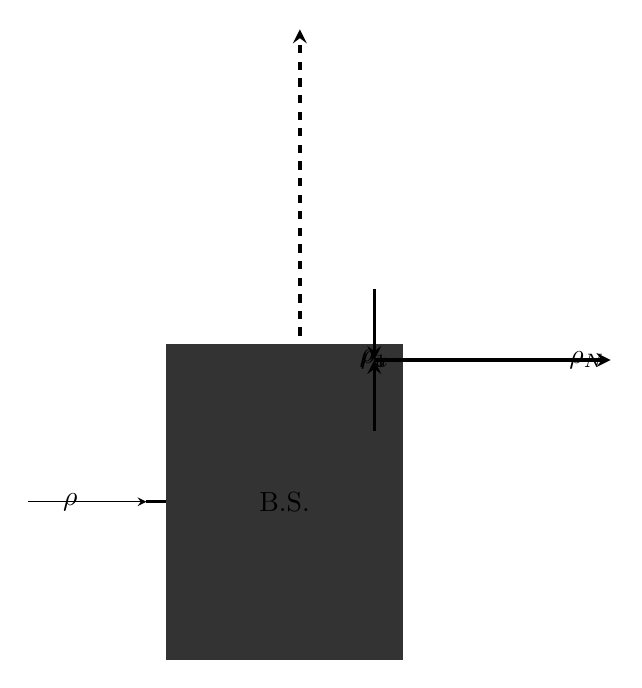
\begin{tikzpicture}[scale=1.5,
    Amp/.style={fill=black, draw=black, minimum width=2cm, minimum height=3cm},
    BS/.style={fill=black!80, draw=black!80, minimum width=3cm, minimum height=4cm},
    >=stealth
  ]

  % Paths
  \draw[->] (-1, 0) -- node[left] {$\rho$} (0, 0);
  \draw[->, very thick] (0, 0) -- (1, 0) coordinate[pos=.9] (AmpStart);
  \draw[->, very thick] (0, 0) -- (1.3, 0) coordinate[pos=.9] (BSStart);
  \draw[->, dashed, very thick] (1.3, 0) -- ++(0, 4) coordinate[pos=.3] (BSEnd);
  \draw[->, very thick] (BSEnd) -- (BSEnd -| 2, 0) coordinate[pos=.9] (BSStop);

  % Nodes
  \node [Amp, draw=black, label=center:Amp] at (AmpStart) {};
  \node [BS, label=center:B.S.] at (BSStart) {};
  \draw[->, very thick] (BSStop) -- ++(2, 0) coordinate[pos=.9] (End);
  \node at (BSStop |- End) (rho1) {$\rho_1$};
  \node at (BSStop |- End -| BSStop) (rhoMu) {$\rho_{\mu}$};
  \node at (BSStop |- End -| BSStop -| End) (rhoN) {$\rho_N$};
  
  % Arrows from output
  \draw[<-, very thick] (BSStop) -- ++(0, .6) node[right] {};
  \draw[<-, very thick] (BSStop) -- ++(0, -.6) node[right] {};

\end{tikzpicture}

\caption{Strategy for establishing the $N$-extendibility of the thermal-noise-channel. The initial state $\rho$ is amplified and split into $N$ modes using a beam splitter. The beam splitter (B.S.) splits the amplified state into two outputs, which are then further split into $N$ modes each. This process illustrates the concept of extending the thermal noise channel to multiple modes.}

\end{document}